Because our study includes individuals who experienced the Reggio Approach as well as others who experienced other early childhood programs, it is important to examine the similarities and differences across the available programs. This section documents the Reggio Approach in addition to exploring the extent to which other programs adopted innovative features of the Reggio Approach at different points of time.

To increase our understanding of the evolution of the programs listed in Table~\ref{tab:itc-pre}, we collected historical records from Reggio Emilia and Padova\footnote{We were unsuccessful in sourcing historical records from Parma.} \citep{Padova-Admin-Data_1964-2011,Reggio-Admin-data_1966-2006,Reggio-Annual-Journals_1994-2011} and administered a survey to current and former school administrators and educative coordinators in order to quantify pedagogical and administrative features of early childhood programs available during 1950-2010 \citep{CEHD_2016_Historical-Analysis}.\footnote{See Appendix~\ref{sec:survey} for the survey.}
~\\
\begin{table}[H]
\centering
\caption{Availability of Preschool Programs by City and School Type}\label{tab:itc-pre}
\begin{adjustbox}{width=\textwidth}
\begin{threeparttable}
	\begin{tabular}{l l c c c c c c c c c}
\toprule
\mc{1}{c}{Cohort} & \mc{1}{c}{Years} & \mc{3}{c}{Reggio Emilia} & \mc{3}{c}{Parma} & \mc{3}{c}{Padova} \\
& & Municipal & Catholic & State & Municipal & Catholic & State & Municipal & Catholic & State \\
\midrule
Adults 50s & 1957-1965 & & \checkmark & & & \checkmark & & & \checkmark & \\
Adults 40s & 1972-1976 & \checkmark & \checkmark & & & \checkmark & & & \checkmark & \\
Adults 30s & 1983-1987 & \checkmark & \checkmark & \checkmark & \checkmark & \checkmark & \checkmark & \checkmark & \checkmark & \checkmark \\
Adolescents & 1994-2000 & \checkmark & \checkmark & \checkmark & \checkmark & \checkmark & \checkmark & \checkmark & \checkmark & \checkmark \\
Children & 2009-2014 & \checkmark & \checkmark & \checkmark & \checkmark & \checkmark & \checkmark & \checkmark & \checkmark & \checkmark \\
\bottomrule
\end{tabular}

% Caption:
% Note: This table indicates the types of educational preschool systems (defined as programs with 4 or more sites) available to parents in each city during the years each cohort was eligible for a 3-6 year old program. 
\begin{tablenotes}
\end{tablenotes}
\end{threeparttable}
\end{adjustbox}
\end{table}

The survey was designed to explore the extent to which the key administrative and pedagogical components of the Reggio Approach were present in each city's state, religious, and municipal systems at different points of time. The components included in the survey were identified by published program descriptions and confirmed by scholars of the Reggio Approach and early childhood programs in Northern Italy.\footnote{See \citet{Edwards-etal-eds_1998_Hundred-Languages} and \citet{Corsaro_2008_Policy-Practice}.} The list of components includes various aspects of administrative program operations such as staffing, supervision, enrollment, and funding. It also considers pedagogy and educational practices for children's learning and parental engagement. Respondents were asked to indicate whether the central features of Reggio were present in their systems during different decades. Additional questions were included to understand a) extent of variation between municipal programs and private providers contracted by the municipality; b) extent of site-level variation within systems; c) perceived variation between similar systems in other cities; d) sources of program funding, and e) services for immigrant families.\footnote{For a more detailed summary of the items and the responses, see Appendix~\ref{sec:survey}.} Table~\ref{tab:respondents} identifies the school systems in each city that completed our survey.

\begin{table}[H]
\centering
\caption{Survey Respondents by City and School Type}\label{tab:respondents}
\begin{threeparttable}
	\begin{tabular}{lccc}
\toprule
City & Municipal & State & Religious \\
\midrule
Reggio Emilia & \checkmark & \checkmark & \\
Parma		& \checkmark & & \\
Padova & \checkmark & \checkmark & \checkmark \\
\bottomrule
\end{tabular}
\begin{tablenotes}
This table indicates the systems represented by survey respondents. These individuals include current and former administrators and educational coordinators. One survey was provided by each system noted, but answers reflected the input of multiple people employed by the system. Responses were provided by religious systems in Reggio Emilia and Parma, however, they do not include historical data prior to 2000.
\end{tablenotes}
\end{threeparttable}
\end{table}

\textbf{[JJH: Question, a separate survey for each program? Sylvi: Yes. Each program reported on their own services separately, and the same survey was sent to all programs, so that everyone was aware we were asking the same set of questions to each.]}

Results from the historical survey indicate that early childhood education systems within Reggio Emilia, as well as in Parma and Padova, share a number of similar characteristics. These include features of program administration, various pedagogical methods, and practices for at-risk children and families. The general trend shows that programming and practices endorsed by the municipality of Reggio Emilia are increasingly present in other early childhood systems, albeit to different degrees and at different times. We interpret these results as evidence supporting spillovers of Reggio features into other early childhood programs. \textbf{[Team: We are cautious about strong claims of spillovers, as our survey data indicates that other programs were not influenced by Malaguzzi or the Reggio Approach.]} We acknowledge the small sample of survey respondents is too limited to ensure reliability or validity of outcomes. We further acknowledge the design of our historical survey limits our ability to capture strengths and uniquenesses of alternative approaches. We caution that the evidence from our survey should not be interpreted as a quality measure of early childhood systems.

To summarize our findings, we compare the different programs in Figures~\ref{fig:agg-admin} and~\ref{fig:agg-ped}. A more detailed description is provided in the section that follows. Using survey results, we calculate the number of administrative and pedagogical components that each program shared with the Reggio Approach by school type, city, and year. We examine 14 administrative components and 16 pedagogical components (not all of the pedagogical components were present in the Reggio Approach). Over time, many of the programs increasingly implemented pedagogical and administrative practices endorsed by the Reggio Approach. This is especially true for Parma's municipal program, and somewhat true for Padova's municipal program. The other systems did not adopt as many pedagogical components as they did administrative ones. Even though the Reggio Approach remains distinctive when considering the sum of its elements, many of the alternative schools evolved to include a substantial portion of the elements in Reggio Emilia's municipal system.

\begin{figure}[H]
\begin{center}
\begin{subfigure}[b]{0.49\textwidth}
	\caption{Number of Administrative Characteristics in Common with the Reggio Approach}\label{fig:agg-admin}
	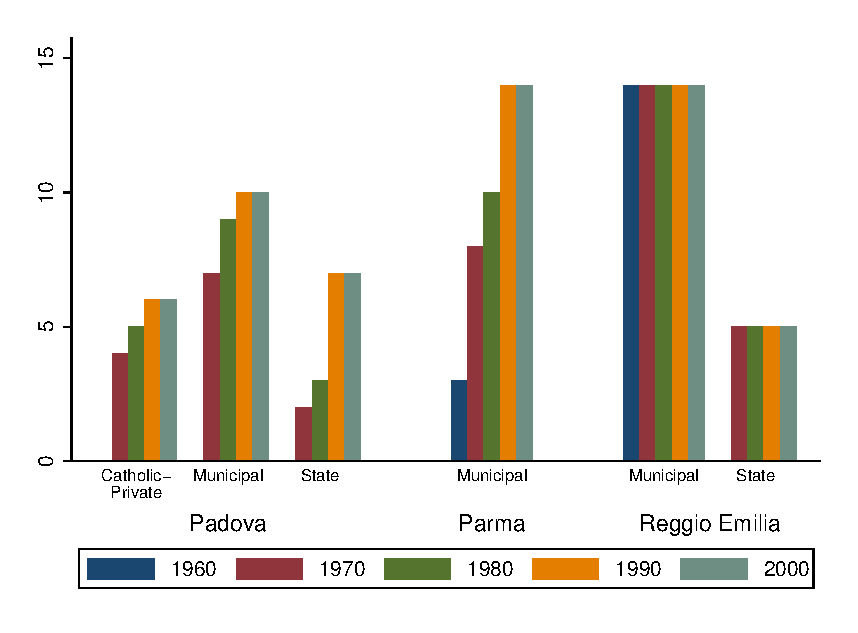
\includegraphics[width=\textwidth]{../../output/aggregateAdministrative.eps}
\end{subfigure}%
~
\begin{subfigure}[b]{0.49\textwidth}
	\caption{Number of Pedagogical Characteristics in Common with the Reggio Approach}\label{fig:agg-ped}
	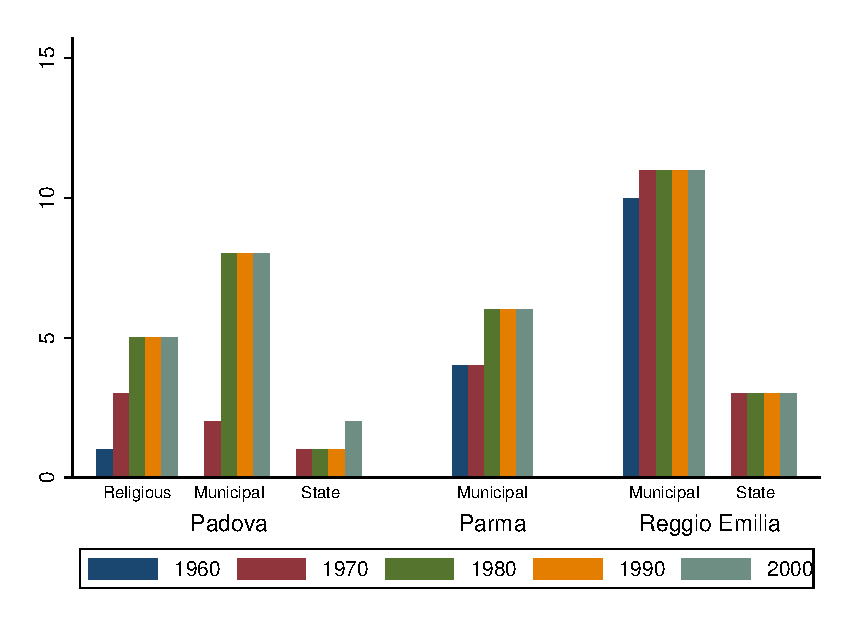
\includegraphics[width=\textwidth]{../../output/aggregatePedagogical.eps}
\end{subfigure}%
\end{center}
\raggedright \footnotesize Note: These graphs show the number of administrative and pedagogical components that each program has in common with the Reggio Approach. We consider 14 administrative components and 16 pedagogical components. Some of the pedagogical components were not present in the Reggio Approach.
\end{figure}

%\footnote{See Appendix~\ref{} for more extensive discussion of the survey results.}

\subsection{Municipal Schools in Reggio Emilia - The Reggio Approach}

Of the municipal systems in Reggio Emilia, Parma, and Padova, the Reggio Approach is notable for innovative programming, investment in staffing, and broad provision of early childhood services. Of the three, it was the earliest municipal system to evolve and historically offers the largest number of municipal infant-toddler and preschool sites.\footnote{Similar to Parma and Padova, Reggio Emilia contracts with local private providers and cooperatives to offer infant-toddler and preschool slots according to municipal regulations. These ``affiliated'' programs may not follow the Reggio Approach nor the municipal approaches in Parma and Padova. Accordingly, we consider this a separate sample during analysis.} Reggio Emilia's municipal early childhood system preceded Italy's key educational reforms of 1968 and 1971 legislating free state preschools and local provision of infant-toddler childcare \citep{Cagliari-etal-eds_2016_BOOK_Loris-Malaguzzi}. 

The Reggio Approach is a form of progressive early childhood education shaped by Loris Malaguzzi, a psychologist and educator influenced by Dewey's model of progressive education, Vygotsky, and psychological theories of Piaget and Erikson. \textbf{[JJH: Do we know this? Sylvi: These four theorists are confirmed by our survey and cited in Cagliari 2016. We also ask about Bronfenbrenner, Kagan, and Gardner as influences on the Reggio Approach in our survey. We propose they appear in the Memo as our survey results indicate their influence on other programs.]} Under Malaguzzi's direction, Reggio Emilia constructed its first preschool for children aged 3-6 years in 1963. In 1965, the municipality legislated funding for infant-toddler centers for children aged 3 to 36 months; the first center opened in 1971. 

In Reggio Approach schools, there is no institutionally-prescribed content knowledge that educators convey to children to achieve the goal of ``school readiness.'' In contrast, curriculum is more methodology than content. Curriculum is viewed as an ongoing, collaborative project between educators, children and families, with emergent learning goals and flexible project timelines. Adults and children are researchers and co-creators of knowledge. For example, adults and children collaborate to define a question or topic. Learning is then pursued following a scientific process: theories are shared, tested, and revised through socratic questions and dialogue. \textbf{[JJH: But this is a method -- select a project and review. Sylvi: I agree. Reggio's curriculum is more method than content (in contrast to state, religious, and the other municipal programs which focus more on content). We now state this more explicitly.]} Children demonstrate their emerging knowledge through expressive art forms, with aid from the atelierista. Teachers document each child's work in a portfolio that is shared with children and parents over the year to observe the child's development \citep{Rinaldi_2006_ReggioEmilia_BOOK,Giudici-Nicolosi_2014_Reggio-Approach}

In Reggio preschools, incoming 3-year old cohorts form a homogenous classroom of about 25 children. Cohorts are assigned two full-time co-teachers (1:12-13). Teachers observe children's development, interact with children through questions and dialogue, and provide scaffolding to support learning. At least 1 of the 2 teachers remains with each cohort for three consecutive years. offering extended time for continuity of care and strong teacher-family engagement. Each preschool site is further staffed by a full-time atelierista, an instructor with a background in visual arts, who helps teachers develop creative learning activities. A pedagogista, or educational coordinator, with a post-BA \textbf{[JJH: Post-BA? Sylvi: Depending on the decade, either a BA or a diploma from a post-high school teaching program.]} in psychology or education is assigned to support professional development on a biweekly basis for the educational staff of approximately 4-5 municipal preschools. Auxiliary site staff, such as cooks and janitors, are considered members of the educational team and participate in the biweekly trainings.

School environments reflect a light-filled, open interior design, furnished with natural materials and a garden. In-house kitchens are surrounded by glass walls, to include children in the meal process, and is used daily for preparing meals. Each preschool is equipped with an atelier, or dedicated studio laboratory, where children and educators collaborate on creative instructional activities.

The engagement of families \textbf{[JJH: What does this mean? What is engagement? Sylvi: Please note revised text.]} is embedded in Reggio Approach practices. Preschools and infant-toddler centers are open five full-time days per week from September through June \citep{Giudici-Nicolosi_2014_Reggio-Approach}. Some sites offer programming in July and extended day options are available at a majority of sites throughout the school year to accommodate working parents. Reggio Approach schools prioritize admission for single parents and children with disabilities \citep{Edwards-etal-eds_1998_Hundred-Languages}. Parents and community members are invited to participate in school management and shape school policies, volunteer in the classroom, and host field trips in the community \citep{CEHD_2016_Historical-Analysis,Cagliari-etal-eds_2016_BOOK_Loris-Malaguzzi}. 

\subsection{Municipal Schools in Parma and Padova}

The municipal early childhood systems in Parma and Padova emerged after Reggio Emilia designed the Reggio Approach. Both systems are currently, and were historically, smaller than that of Reggio Emilia. Parma's municipal early childhood system consolidated and expanded around 1975, about a decade after that of Reggio Emilia. While Padova offered five municipal sites by 1976, investment into high quality educational programming by the municipality did not occur until the mid-1980s. For additional information, see (see Appendix Table~\ref{tab:educ-program}). 

Although the municipal systems in Parma and Padova are somewhat different from each other and from the municipal schools in Reggio Emilia, they share many features. The results from the survey indicate that the municipal schools in Parma and Padova also assigned importance to helping at-risk families\footnote{These families include those of a low economic status, those with a single parent, and children with a disability.} by offering services that helped such families (e.g., offering extended hours) and by prioritizing enrollment for children from these families (see Appendix Table~\ref{tab:administrative-atrisk}). 

Starting in the 2000s, Parma and Padova's municipal systems were influenced by the same academic theories of psychology and early childhood education as Reggio Emilia and teachers began to document children's learning (see Appendix Table~\ref{tab:educ-program}). However, the municipal systems in Parma and Padova differ considerably from the Reggio Approach in the implementation of these theories. In Parma and Padova's municipal systems, religious instruction is provided. Furthermore, a pre-defined program is implemented to guide children in learning specific concepts such as communication, culture, order, measure, space, time, nature, self, and other \textbf{[JJH: Such as? Sylvi: The program concepts are intentionally vague in order to be actualized at the individual school-level, similar to Head Start. (In contrast, in Reggio, chosen concepts are not pre-determined but follow the child's lead.)]} Neither of these educational components are present in the Reggio Approach (see Appendix Table~\ref{tab:educ-program}).  \textbf{[JJH: Why inconsistent? Sylvi: Apologies, I'm unsure what inconsistency you refer to.]}. 

\subsection{State Preschools}

State preschools are mandated by 1968 law regarding the provision and funding of free, public preschools -- only where local demand was not already met by existing non-state systems \citep{Hohnerlein_2009_Paradox-Public-Preschools}.\footnote{In state programs, parents pay only for meals, transportation, and extras such as field trips and extracurricular lessons. Although the state does not offer infant-toddler childcare, it regulates and subsidizes these programs through regional governments.} This policy resulted in disparate numbers of state preschools in Reggio Emilia, Parma, and Padova for each of the cohorts in our evaluation. Historical records indicate that state preschools first appeared in Reggio Emilia and Padova between 1973-1975 \citep{Padova-Admin-Data_1964-2011,Reggio-Admin-data_1966-2006,Reggio-Annual-Journals_1994-2011}. In contrast to other areas of Italy where the state is currently the largest provider of preschool education, enrollment in Reggio Emilia, Parma, and Padova's state preschools has historically lagged behind municipal and religious programs.

Reports suggest that policies and guidelines for state schools, Orientamenti, were historically influenced by municipal programs from the region of Emilia Romagna, including Reggio Emilia, Milan, and Pistoia \citep{OECD_2001_Italy-Country-Note}. Periodic improvements to state Orientamenti, along with revised mandates for lower teacher-child ratios and higher qualifications for teacher education, are proposed as key quality indicators associated with diminishing disparities in state and non-state programs by the end of the 20th century \citep{Hohnerlein_2015_Development-and-Diffusion}. For example, teacher-child ratios were very low for the three adult cohorts ranging from 27 to 36 children aged 3-5 years per teacher \textbf{[JJH: At what age and over what period? Sylvi: We have revised the text to answer these questions]}. Attendees of state preschools in the adolescent cohort experienced a 1:17 teacher-child ratio. In the child cohort, teacher-child ratios in state preschools was equivalent to that of the Reggio Approach \citep{Hohnerlein_2015_Development-and-Diffusion}.

The results from the survey indicate that the programming and operations of state preschools in Reggio Emilia are different from the Reggio Approach and municipal programs in Parma, and Padova. State preschools do not offer extended hours to working families, thus state teachers work shorter hours than their municipal counterparts. State preschools do not have full-time Pedagogistas to oversee programs, do not have an expert in the creative arts, and do not set aside time for teachers to engage families (see Appendix Table \ref{tab:programoperation}). Moreover, state preschools in Reggio Emilia have a different approach to support children's learning compared to the Reggio Approach in that the program is  influenced by different academic theories, religious teaching is provided, and daily activities follow a program to guide children in learning of specific concepts. In contrast, the Reggio Approach is based on research-based projects with unlimited timelines (see Appendix Table~\ref{tab:educ-program}). The survey results also indicate that state preschools in Padova are similar to those in Reggio Emilia, except that they provided professional development from the 1990s (see Appendix Tables~\ref{tab:programoperation} - \ref{tab:environ-features}).

\subsection{Religious Preschools}

The Catholic Church is the oldest early childhood provider in Italy, offering both religious training and charitable social services for disadvantaged children since the 19th century \citep{OECD_2001_Italy-Country-Note}. While the Church does not offer educational infant-toddler programs, as in the Reggio Approach, nor implement a unified system of religious preschool education, religious institutions began to assemble local federations in the mid-1970s. Within federations, distinct religious sites are enabled to offer independent programs.

Following a 1997 policy providing state funding for non-state programs (i.e., municipal and religious) that met national guidelines for early childhood, the Catholic Church undertook significant efforts to quantify and achieve equitable program quality \citep{Malizia-Cicatelli_2011_BOOK_Catholic-School}. For example, religious educators were replaced with secular teachers trained in higher institutions and teacher-child ratios were greatly reduced to reflect national standards. Parents of the youngest cohort in our sample, born in 2006, who enrolled in equitable religious programs were eligible for subsidized tuition on a sliding-scale basis, and their children experienced educational programming that reflected an influence by municipal systems in Emilia Romagna, including Reggio Emilia \citep{Hohnerlein_2009_Paradox-Public-Preschools,OECD_2001_Italy-Country-Note}. For example, while religious programs historically did not provide infant-toddler education, by the late 1990's, some sites in each of the three cities began to offer transitional programming for children aged 24 months \citep{Malizia-Cicatelli_2011_BOOK_Catholic-School,CEHD_2016_Historical-Analysis}.

Survey results for religious preschools are only available for Padova. It is shown that religious preschools in Padova share following the components in program operations with the Reggio Approach: from the 1970s, weekly time is set aside for teachers to engage families \textbf{[JJH: How and for how long? Sylvi: We don't have this data for the 70s and 80s. For the 90s and 2000s, by keeping teachers with the same cohort for 3 years and through ``parental education' (which is undefined). The amount of weekly time is unknown.]}, and from 1980s, for teachers to document children's work. Parental boards are actively engaged in the school culture from the 1970s (see Appendix Table \ref{tab:programoperation}). Padova's religious schools give priority to enrollment to children with disabilities since the 1990s, but they do not prioritize the enrollment of children from economically disadvantaged families, which is unlike the Reggio Approach (see Appendix Table \ref{tab:administrative-atrisk}). Padova's religious schools have an atelier from the 1980s (see Appendix Table \ref{tab:environ-features}). However, unlike the Reggio Approach, Padova's religious preschools provide religious teaching and follow a daily program to guide children in learning specific concepts (see Appendix Table \ref{tab:educ-program}).

